%%%%%%%%%%%%%%%%%%%%%%%%%%%%%%%%%%%%%%%%%%%%%%%%%%%%%%%%%%%
% --------------------------------------------------------
% Rho
% LaTeX Template
% Version 2.1.1 (01/09/2024)
%
% Authors: 
% Guillermo Jimenez (memo.notess1@gmail.com)
% Eduardo Gracidas (eduardo.gracidas29@gmail.com)
% 
% License:
% Creative Commons CC BY 4.0
% --------------------------------------------------------
%%%%%%%%%%%%%%%%%%%%%%%%%%%%%%%%%%%%%%%%%%%%%%%%%%%%%%%%%%%

\documentclass[9pt,a4paper,twoside]{rho-class/rho}
\usepackage[english]{babel}

%% Spanish babel recomendation
% \usepackage[spanish,es-nodecimaldot,es-noindentfirst]{babel}

\setbool{rho-abstract}{true} % Set false to hide the abstract
\setbool{corres-info}{false} % Set false to hide the corresponding author section

%----------------------------------------------------------
% TITLE
%----------------------------------------------------------

\title{Refactored Implementation and Validation of the Two-Component Power Law Phase Screen Model for GNSS Ionospheric Scintillation Simulation}

%----------------------------------------------------------
% AUTHORS AND AFFILIATIONS
%----------------------------------------------------------

\author[1]{Rodrigo de Lima Florindo}

%----------------------------------------------------------

\affil[1]{Aeronautics Institute of Technology (ITA), São José dos Campos, SP, Brazil.}

%----------------------------------------------------------
% FOOTER INFORMATION
%----------------------------------------------------------

%\leadauthor{Author last name et al.}
\institution{Aeronautics Institute of Technology (ITA), São José dos Campos, SP, Brazil.}
\theday{May 21, 2024} %\today

%----------------------------------------------------------
% ARTICLE INFORMATION
%----------------------------------------------------------

\corres{Provide the corresponding author information and publisher here.}
\email{example@organization.com.}
\doi{\url{https://www.doi.org/exampledoi/XXXXXXXXXX}}

\received{March 20, 2024}
\revised{April 16, 2024}
\accepted{April 20, 2024}
\published{May 21, 2024}

\license{Rho LaTeX Class \ccLogo\ This document is licensed under Creative Commons CC BY 4.0.}

%----------------------------------------------------------
% ABSTRACT
%----------------------------------------------------------

\begin{abstract}
    Ionospheric scintillation affects GNSS signals, causing rapid amplitude and phase variations that degrade receiver performance. The Two-Component Power Law Phase Screen Model (TPPSM) provides a statistical framework for simulating these effects. However, existing implementations lack support for simultaneous weak scattering simulations and real satellite orbits, while also suffering from poor documentation and organization. This study presents a refactored TPPSM implementation, improving code structure, readability, and flexibility for modeling weak, moderate, and severe scintillation conditions. The refactored version is validated through spectral comparisons, showing strong agreement between simulated and theoretical intensity and phase spectra. A systematic methodology is proposed for generating scintillation time series, incorporating receiver motion, multi-frequency scaling of irregularity parameters, and realistic ionospheric conditions. Although currently limited to rectilinear receiver trajectories, future extensions could accommodate arbitrary motion, benefiting applications such as aerospace navigation, ionospheric monitoring, and GNSS signal resilience studies.
\end{abstract}

%----------------------------------------------------------

\keywords{Ionospheric scintillation, GNSS, Phase screen model, TPPSM, Ionospheric irregularities, Weak and Strong scattering, Scintillation time series, GNSS signal propagation.}

%----------------------------------------------------------

\begin{document}
	
    \maketitle
    \thispagestyle{firststyle}
    % \tableofcontents
    %\linenumbers

%----------------------------------------------------------
\section{Introduction} 
\label{sec:introduction}
The purpose of this report is threefold:
\begin{itemize}
    \item To synthesize the key aspects of the TPPSM, which are currently scattered across  multiple journal articles, conference papers and books.
    \item To present preliminary results validating a newly refactored code with improved documentation, readability and organization. This refactored code was developed based on the two publicly available TPPSM implementations provided by the Colorado Boulder group on Github.
    \item To stablish a methodology that could be used to generate relevant scintillation time series using the TPPSM.
\end{itemize}
Section \ref{sec:ps_theory} provides a concise review of the phase screen and wave propagation theory underlying the TPPSM.  Section \ref{sec:irregularity_parameter_estimation} presents a brief literature review on the estimation of irregularity parameters used by the TPPSM, highlighting those relevant for generating scintillation time series.  we assess the validity of the time series generated by the proposed refactored TPPSM by comparing their intensity and phase spectra with the expected theoretical shapes provided by a code developed for analyzing the two-component power-law morphology described in \cite{Carrano2016OverviewOfTwoComponentPowerLaw}. Section \ref{sec:time_series_methodology} proposes a general methodology for generating meaningful scintillation time series for different applications. Finally, Section \ref{sec:conclusions} summarizes the main findings of this work.
\section{Phase Screen Realizations and Wave Propagation}
\label{sec:ps_theory}

The amplitude and phase distortions caused by a random ionosphere medium on a wave propagating from a GNSS satellite to a receiver plane is governed by the parabolic wave equation (PWE) \cite{rinoCompactMultifrequencyGNSS2018} \cite{rinoTheoryScintillationApplications2011} \cite{vasylyevModelingIonosphericScintillation2022}.

Considering that the ionospheric irregularities are usually enlongated along the magnectic field line \cite{SizeShapeOrientationOfEquatorialAnomalyScintillations}, we can neglect the distortions caused by the ionosphere medium on the north-south direction for equatorial regions \cite[Section III]{JiaoMultifrequencyScintillationOnGPSSignalsStaticPlatforms2018}. Thus, a continuous scalar form of the PWE is sufficient to describe the interaction of the GNSS propagated signal through the ionosphere and its diffractive pattern seen on the observer plane, which can be given by \cite[Equation 6]{rinoCompactMultifrequencyGNSS2018}:
\begin{align}
    \label{eq:PWE}
    \frac{\partial \psi\left( x, y \right)}{\partial x} = \Theta_{\rho_F} \psi \left( x, y \right) + j k \Delta n \left( x, y \right) \psi \left( x, y \right) \text{.}
\end{align}
where $x$ is the downward direction normal to the ionosphere layer and $y$ is the geomagnectic eastward, $\psi\left( x, y \right)$ is the principal component of the propagated electromagnetic field, $\Theta_{\rho_F} \psi \left( x, y \right)$ represents the free-space propagation, which is related to the diffraction pattern observed in the receiver plane, where the $\Theta_{\rho_F}$ operator is defined in \cite[Equation 7 and 8]{rinoCompactMultifrequencyGNSS2018} and $j k \Delta n \left( x, y \right) \psi \left( x, y \right)$ denotes the refraction of the propagated signal caused by its passage through the ionosphere medium. Furthermore, $k=2\pi f_c/c$ is the transmitted signal wavenumber and $\Delta n\left( x, y \right)$ symbolizes a local pertubation on the refractive index. Figure \ref{fig:propagation_geom} shows the geometric configuration of a GNSS signal oblique propagation.
\begin{figure}
    \centering
    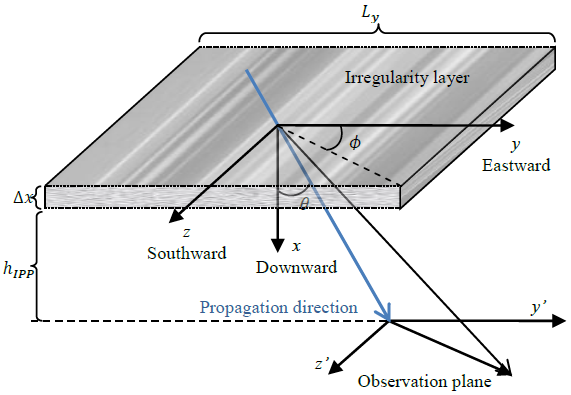
\includegraphics[width=0.45\textwidth]{figures/Propagation Geometry - Yu Jiao.png}
    \caption{Propagation geometry of the scintillation signal. This figure was copied from Figure 2 of \cite{JiaoMultifrequencyScintillationOnGPSSignalsStaticPlatforms2018}}
    \label{fig:propagation_geom}
\end{figure}

A widely adopted solution for the equation \eqref{eq:PWE} is known as the split-step algorithm, which alternates between generating a discrete realization of the phase shift related to the propagated signal refraction in the ionosphere medium and the computation of the free-space propagation effects \cite{rinoTheoryScintillationApplications2011}. In general, to obtain a meaningful scintillation signal, it is necessary to iterate the split-step algorithm through multiple phase screens \cite{vasylyevModelingIonosphericScintillation2022}. However, as was argued in \cite{rinoCompactMultifrequencyGNSS2018}, it is possible to replace the usage of multiple phase screens by a single \textit{equivalent} phase screen for equatorial scintillation events. 

The split-step algorithm can be summarized by the pair of discrete equations \eqref{eq:fft_phase_realization} and \eqref{eq:free_space_propagation} \cite[Equations 1 and 2]{xuTwoparameterMultifrequencyGPS2020}:
\begin{align}
    \label{eq:fft_phase_realization}
    \Psi\left[ 0; n \right] = \sum^{N-1}_{m=0}{\exp\left\{ j \phi\left[ m \right] \right\} \exp\left\{ -2\pi j n m / N \right\}} \text{;}
\end{align}
\begin{align}
    \label{eq:free_space_propagation}
    \psi\left[ x; m  \right] = \frac{1}{N}  \sum^{N-1}_{n=0} \Psi\left[ 0; n \right]
    &\exp \left\{ -j k \left( n \Delta q / k \right)^2 x / 2 \right\} \times \notag \\ 
    \times & \exp\left\{ 2 \pi j n m / N \right\} \text{,}
\end{align}
where $\Psi \left[ 0; n \right]$ represents a $N$-size discrete Fourier transform (DFT) of a complex signal $\exp\left\{ j \phi\left[ m \right] \right\}$ with a unitary amplitude and a phase characterized by the signal $\phi\left[ m \right]$, which is generated from a modeled spectral density function (SDF) with a resolution of discrete samples of $\Delta y$. In addition, $q$ denotes the spatial frequency in the $y$ direction with $\Delta q$ being its resolution.

After substituing the value of $x$ by the Fresnel scale
\begin{align}
    \rho_F = \sqrt{x/k} \text{,}
\end{align}
the equation \eqref{eq:free_space_propagation} can be further simplified as
\begin{align}
    \label{eq:free_space_propagation_simplified}
    \psi\left[ \rho_F; m \right] = \frac{1}{N} \sum_{n=0}^{N-1} \Psi\left[ 0; n \right]
    & \exp \left\{ -j\left( n\Delta q \rho_F \right)^2 /2 \right\} \times \notag \\
    \times & \exp \left\{ 2\pi j n m /N \right\}
\end{align}

As proposed in \cite{rinoCompactMultifrequencyGNSS2018}, a realistic path-integrated phase realization can be obtained from a one-dimensional two-component power law SDF, which can be defined as
\begin{align}
    \label{eq:original_SDF}
    \Phi_{\phi}\left( q \right) = C_p 
    \begin{cases} 
        q^{-p_1}, & q \leq q_0 \\ 
        q_0^{p_2 - p_1} q^{-p_2}, & q > q_0
    \end{cases}
\end{align}
where $q_0$ denotes the spatial wavenumber at which the power-law index change from $p_1$ to $p_2$, and $C_p$ is the turbulence strength \cite[Description below equation 5]{JiaoScintillationOnGPSSignalsForDynamicPlatforms2018}.

It is possible to simplify the equation \eqref{eq:original_SDF} by normalizing the spatial frequency by the fresnel scale, using $\mu = q \rho_F$. With that, we can rewrite the phase SDF as \cite[Equation 6]{JiaoScintillationOnGPSSignalsForDynamicPlatforms2018}
\begin{align}
    P\left( \mu \right) = \Phi_{\phi}\left( q \right) / \rho_F = 
    \begin{cases} 
        U_1 \mu^{-p_1}, & \mu \leq \mu_0 \\ 
        U_2 \mu^{-p_2}, & \mu > \mu_0
    \end{cases}
\end{align}
where $U_1 = C_p \rho_F^{p_1 - 1}$ and $U_2 = C_p \rho_F^{p_1 - 1} \mu_0^{p_2 - p_1}$. It is important to comment here that some papers uses the symbol $C_{pp}$ instead of $U_1$ \cite[Equation 21]{a rinoCompactMultifrequencyGNSS2018}. Therefore, the so-called universal scattering strength $U$ can be defined as \cite[Equation 7]{JiaoScintillationOnGPSSignalsForDynamicPlatforms2018}
\begin{align}
    U =
    \begin{cases}
        C_{pp} = U_1, & \mu_0 \geq 1 \\
        U_2, & \mu_0 < 1
    \end{cases} \text{,}
\end{align}
where $U_2 = U_1 \mu_0^{p_2-p_1}$. With that, we can observe that $U$ is the normalized phase spectral power at $\rho_F$, given that $U \equiv P\left( \mu = 1 \right)$ \cite{Carrano2016OverviewOfTwoComponentPowerLaw}. When $U \ll 1$, the scatter is weak, and when $U \gg 1$, the scatter is strong \cite{Carrano2016OverviewOfTwoComponentPowerLaw}. 

In order to extend the irregularity parameters obtained for a specific frequency band to others, a scaling approach is applied. Since ionospheric scintillation parameters are frequency-dependent, their values for a frequency band $f_2$ are derived by adjusting those from $f_1$ using a frequency ratio factor. This ensures consistency in parameter estimation across different frequencies.

The normalized break wavenumber parameter at a frequency band $f_2$, denoted as $\mu_{0,f_2}$, is scaled from a frequency band $f_1$ using the relation \cite[Equation 17]{JiaoScintillationOnGPSSignalsForDynamicPlatforms2018}:
\begin{equation}
    \label{eq:mu0_extrapolation}
    \mu_{0,f_2} = \mu_{0,f_1} \sqrt{f_1 / f_2}
\end{equation}

Similarly, an extrapolated time-scaling parameter, ${\rho_F / v_{eff}}_{f_2}$, is given by \cite[Equation 18]{JiaoScintillationOnGPSSignalsForDynamicPlatforms2018}:
\begin{equation}
    \label{eq:rhoFveff_extrapolation}
    {\rho_F / v_{eff}}_{f_2} = {\rho_F / v_{eff}}_{f_1} \sqrt{f_1 / f_2}
\end{equation}

Lastly, the universal turbulence strength parameter $U_{f_2}$ is extrapolated from $U_{f_1}$ using the following piecewise relation \cite[Equation 19]{JiaoScintillationOnGPSSignalsForDynamicPlatforms2018}:
\begin{equation}
    \label{eq:U_extrapolation}
    U_{f_2} =
    \begin{cases} 
        U_{f_1} \left(f_1 / f_2\right)^{0.5p_1 + 1.5}, &\mu_{0,f_1} \geq 1, \mu_{0,f_2} \geq 1 \\
        U_{f_1} / \mu_{0,f_1}^{p_2-p_1} \left( f_1 / f_2 \right)^{0.5 p_1 + 1.5}, & \mu_{0,f_1} < 1, \mu_{0,f_2} \geq 1 \\
        U_{f_1} \left( \mu_{0,f_2} / \mu_{0,f_1} \right)^{p_2 - p_1} \left(f_1 / f_2\right)^{0.5 p_1 + 1.5}, & \mu_{0,f_1} < 1, \mu_{0,f_2} < 1
    \end{cases}
\end{equation}

It is important to emphasize here that the equations \eqref{eq:mu0_extrapolation}, \eqref{eq:rhoFveff_extrapolation} and \eqref{eq:U_extrapolation} are derived based on weak scintillation theory and serve as approximations in strong scattering conditions \cite{Rino1979WeakScatter}.

A comprehensive analysis of the two-component power law spectra can be found in \cite{Carrano2016OverviewOfTwoComponentPowerLaw}. This work underpinned the importance of understanding the physical meaning of this kind of spectral model, which also nests a widely used one-component power law model \cite{CarranoBrazil2012}. The two-component power law model can be modeled in such manners that it captures the electron density statistical properties of the inner and outer scales that defines the complete ionosphere structure. With that, this spectra is well-suited for modeling weak and strong signal scattering caused on the ionosphere medium.

A Statistically equivalent phase screen realization $\overline{\phi}\left[ m \right]$ can be obtained by imposing $P\left( \mu \right)$ on a complex Gaussian random variable $\eta\left[ n \right] \sim \mathcal{C N}\left( 0, 1 \right)$ with the Hermitian and the white noise properties \cite{rinoCompactMultifrequencyGNSS2018}
\begin{align}
    \eta\left[ n \right] = \text{mod}\left( \eta^*\left[ N \right], N \right) \text{,} \\
    \mathbb{E}\left\{ \eta\left[ n \right] \eta^{*}\left[ n' \right] \right\} = \delta\left[ n-n' \right] \text{,}
\end{align}
respectively, where $mod\left( \cdot \right)$ denotes the modulus operator and $E\left\{ \cdot \right\}$ represents the expectation. Thus, we have
\begin{align}
    \label{eq:phase_screen_realization}
    \overline{\phi}\left[ m \right] = \sum_{n=0}^{N-1} \sqrt{P(n\Delta \mu) \Delta \mu / (2\pi)} \, \eta\left[ n \right] \exp\{-2 \pi j n m / N\} \text{.}
\end{align}
It is worthy to clarify that this equation represents an inverse discrete Fourier Transform (IDFT). Note here that the term $1/N$ that commonly appears in a IDFT is related to $\Delta \mu$ in this equation, which in its part is related to the variable of integration of the IDFT. Please refer to \cite[Section 6.1]{vasylyevModelingIonosphericScintillation2022} and \cite[Section 2.2.4]{rinoTheoryScintillationApplications2011} for further details on the generation of phase realizations based on a defined SDF.

The split step algorithm can be implemented considering equations \eqref{eq:idft_phase_realization_simplified} and \eqref{eq:free_space_propagation_simplified} using a phase realization generated by equation \eqref{eq:phase_screen_realization} as \cite[Equations 9 and 10]{JiaoScintillationOnGPSSignalsForDynamicPlatforms2018}
\begin{align}
    \label{eq:idft_phase_realization_simplified}
    \Psi\left[ 0; n \right] = \sum^{N-1}_{m=0}{\exp\left\{ j \overline{\phi}\left[ m \right] \right\} \exp\left\{ -2\pi j n m / N \right\}} \text{,}
\end{align}
\begin{align}
    \label{eq:post-prop_scint_field}
    \psi\left[ \rho_F; m \right] = \frac{1}{N} \sum_{n=0}^{N-1} \Psi\left[ 0; n \right]
    & \exp \left\{ -j\left( n\Delta \mu \right)^2 /2 \right\} \times \notag \\
    \times & \exp \left\{ 2\pi j n m /N \right\} \text{.}
\end{align}

Furthermore, conversion of the complex field from the space domain to the time domain can be achieved by using a effective scan velocity $v_{eff}$, such that $y\left[ 1 \right] - y\left[ 0 \right] = v_{eff} \left( t\left[ 1 \right] - t\left[ 0 \right] \right)$ \cite[Equation 11]{JiaoMultifrequencyScintillationOnGPSSignalsStaticPlatforms2018}. The effective scan velocity is computed using knowledge of the velocity of the ionospheric piercing point (IPP), the ionosphere mean drift velocity (Which ranges between 25 m/s and 125 m/s \cite{SizeShapeOrientationOfEquatorialAnomalyScintillations} \cite{Wang2017IonoDriftHighLatitude}) and the anisotropy coefficients related to the expected shapes of the ionosphere turbulent media. The reader is referred to \cite[Section 4]{JiaoScintillationOnGPSSignalsForDynamicPlatforms2018} and \cite[Chapter 4]{rinoTheoryScintillationApplications2011} for further details on the computation of $v_{eff}$.

It is worthy to comment for completness here that there are many ways of computing the IPP location for mutually known receiver position and satellite orbit. A comparative study of the most used methods can be found in \cite{Prol2017_Comparative_Study}. 

In addition, it is possible to observe at the file \textit{.../Libraries/PropGeomCalc/PropGeomCalc.m} available at the github repository \url{https://github.com/cu-sense-lab/gnss-scintillation-simulator_2-param} uses the fixed values for the anistropy coefficients $a=50$, $b=1$ and $\gamma_b = 0$. In order to avoid compromising the feasibility of the assumption that the PWE only depends on the eastward direction $y$, i.e., that the change in the refractive index in the southward direction $z$ is negligible, it is better not to change these values, either for the weak and strong scattering cases. The reader is referred to \cite{Vasylyev2024WeakScatterAnisotropy} for details on the ionospheric turbulences anisotropy. 

Considering \cite[Equation 2-14]{harrington2001time} and \cite[The text before equation 26]{rinoCompactMultifrequencyGNSS2018}, we may state the following relation:
\begin{align}
    q &= 2 \pi f_D / v_{eff} \big|_{\times \ \rho_F} \ \therefore \notag \\
    \therefore \ \Delta \mu &= 2 \pi \Delta f_D \rho_F / v_{eff} \text{,}
\end{align}
where $f_D$ represents the Doppler frequency shift related to the effective scan velocity, and $\Delta f_D = 1/\left( N \Delta t \right)$ correponds to the resolution of the samples of the Doppler frequency, where $\Delta t$ denotes the sampling time of the scintillation complex field simulation. It is important to emphasize here that $f_D$ is not directly related to the phase shift caused by receiver-satellite line-of-sight range dynamics. For further detailing of the meaning of $f_D$, please refer to \cite[Text before equation 5]{carrano2017maximum}.

Summarizing, a GNSS complex field scintillation time series can be generated by specifying the irregularity parameters $U$, $p_1$, $p_2$ and $\mu_0$, the time scaling factor $\rho_F / v_{eff}$, which depends only on the satellite-ionosphere-receiver propagation geometry and the sampling parameters $\Delta t$ and $N$. The next section will review how prior studies have proposed to estimate these parameters.
\section{Irregularity Parameter estimation}
\label{sec:irregularity_parameter_estimation}
The generation of realistic ionospheric scintillation effects with the approach described in section \ref{sec:ps_theory} depends entirely on the choice of the aforementioned irregularity parameters. In this view, recent studies have proposed different manners of estimating these parameters by matching a modeled intensity SDF with a real (measured) intensity SDF from a GNSS receiver. 

However, in the lack of real data to fully characterize the irregularity parameters for both weak, moderate and strong scintillation cases, researchers can also choose these parameters based on the comprehensive evaluation of the two-component power law spectred done in \cite{Carrano2016OverviewOfTwoComponentPowerLaw}.
\subsection{Brief Literature Review}

\textcite{CarranoBrazil2012} have initially proposed and evaluated a irregularity parameter estimation (IPE) technique based on a iterative algorithm for evaluating the turbulance strength parameter and the spectral index of a one-component power law model, as well as the zonal drift of the ionosphere. This algorithm relies on the minimization of a metric that measures similarity degree between a modeled and a realistic signal intensity SDF, obtained via detrended real data, by using a downhill simplex algorithm. 

This algorithm was also used in recent works that evaluates the quality of a two-component power-law model in representing the statistics of real ionospheric scintillation events for static \cite{JiaoMultifrequencyScintillationOnGPSSignalsStaticPlatforms2018} and dynamic platforms \cite{JiaoScintillationOnGPSSignalsForDynamicPlatforms2018}. In addition, the work \cite{xuTwoparameterMultifrequencyGPS2020} was also developed using the iterative IPE.

It is important to mention that \textcite{carrano2017maximum} recently presented a more robust solution that is based on maximum likelihood estimation of the irregularity parameters, which was further used to characterize the intermadiate-scale ionospheric structure in \cite{Carrano2018IntermadiateScaleCharacterization}. The author justify that this approach is more robust on the argument that the previous one relies on the Gaussianity and uncorrelatedness of the residuals, while this novel one provides a more comprehensive solution, since this assumption is no longer necessary.

Therefore, since only few algorithms irregularity parameter estimation algorithms were developed, and most of them only tries to find them by fitting a modeled intensity spectrum in a real received signal intensity spectrum, and completly neglects the phase spectrum in this task, there is a necessity of the development of more reliable and computationally efficient algorithms that don't make restricting prior assumptions, such as linearity of the variables.

In order to facilitate the usage of the TPPSM for researchers that are not familiar with phase screen models, \cite{xuTwoparameterMultifrequencyGPS2020} proposed the usage of mapping functions that relates the universal turbulance strength $U$ and the time scaling parameter $\rho_F / v_{eff}$ to the widely used scintillation indices $S_4$ and the $\tau_0$, which are related to the scintillation severity and the decorrelation time, respectively. This work analyzed a large data set of recorded GNSS signals during scintillation events that happened at Ascension Island and Hong Kong.

Despite the usefulness of this approach for simulating moderate and severe ionospheric scintillation events, it is not well-suited for simulating low-intensity ionospheric scintillation events, since the proposed mapping methodology only comprehends $S_4$ values that ranges from 0.5883 to 1.001 \cite[\textit{Libraries/Utilities/ParaMapping.m}]{githubGitHubCusenselabgnssscintillationsimulator_2param}. After testing the model for mild scintillation cases of $S_4$ ($S_4 < 0.3$), negative values of the universal strength parameter $U$ were obatined, which might lead to unrealistic ionospheric scintillation scenarios. An example is shown in figure \ref{fig:low_scintillation_test}.

Therefore, if one wants to use the TPPSM framework to simulate scintillation for any level severity, it is mandatory to apply the direct values of the irregularity parameters by either using a prior study at hand, or obtain them by processing real intensity data using an IPE algorithm.

\begin{figure}
    \centering
    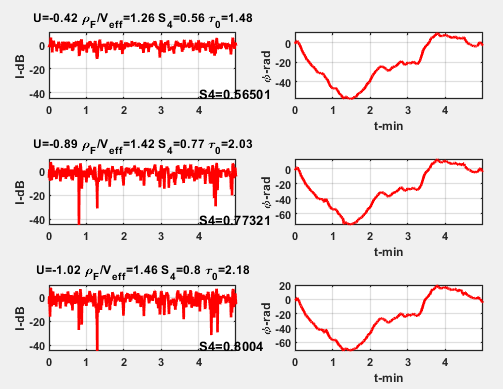
\includegraphics[width=0.40\textwidth]{figures/Low_intensity_test.png}
    \caption{Amplitude and phase scintillation time series obtained from the current version of the two-parameter scintillation model available at \url{https://github.com/cu-sense-lab/gnss-scintillation-simulator_2-param}, for a receiver positioned at Hong Kong (\texttt{userInput.RXPos = [0.3876 1.9942 59.6780]}), moving at 100 m/s at the eastward direction (\texttt{userInput.RXVel = [100 0 0]}), at 10:00:00 UTC in the date 2014/01/02, for the PRN number 18. The chosen values of $S_4$ and $\tau_0$ were 0.2 and 0.7, respectively.}
    \label{fig:low_scintillation_test}
\end{figure}

\subsection{Common Values for Irregularity Parameters for Weak and Strong Scattering}
\label{subsec:common_values_irr_param}
It is possible to observe from \cite[Section 4.4, Figures 7a, 7b, 8a, 8b]{Carrano2016OverviewOfTwoComponentPowerLaw} that, for the case of a one-component power law (named in this study as the \textit{unmodified power law}), the values of scintillation intensity index varies within the range $0.2 < S_4 < 0.4$ and the normalized intensity correlation length $\xi = \xi_c = r / \rho_F$, where $r=r_c$ is defined as the spatial separation for which the intensity correlation decreases to 50\%, varies from $0.2 < \xi_c < 2 s$ for the case when $U = 0.1$ for the values of spectral index within $1.5 < p < 4.5$. Therefore, we can consider $U < 0.1$ and $p=3$ as a feasible set of irregularity parameters for the weak scattering regime (note that there is no spectral break in the one-component power law model).

In addition, it is important to emphasize here that there is a high degree of similarity for the values of $S_4$ and $\xi_c$ in the limiting cases of the two-component power law depicted by \cite[Section 4.4, Figures 7c, 7d, 7e, 7f, 8c, 8d, 8e, 8f]{Carrano2016OverviewOfTwoComponentPowerLaw}, given that $U = U_1 = U_2 \ll 1$. Thus, it is justified the usage of a one-component power law model for this case.

Interestingly, in \cite[Section 4.1]{Carrano2016OverviewOfTwoComponentPowerLaw}, it is noted that the case when $p = 3$ characterizes the least intensity spectral widening and the longest correlation length scenario.

According to \cite{xuTwoparameterMultifrequencyGPS2020}, after using the iterative IPE, it was found that the mean values for $\left\{ \mu_0, p_1, p_2 \right\}$ for the strong scattering regime were 0.55, 2.45 and 3.7, respectively. It is possible to observe the distribution of the estimated parameters at the figure 5 of this same study. In this case, according to \cite[section 3.2.3]{Carrano2016OverviewOfTwoComponentPowerLaw}, this characterizes it as "Mixed-Slope" spectra, where both outer and inner scale structures contribute mutually with distortions to the transmitted signal. Furthermore, it is possible to observe in \cite[Figure 6]{xuTwoparameterMultifrequencyGPS2020} that a value of $U=2$ generates a intensity spectra whose $S_4$ is approximately 0.9, which can be characterized as a severe scintillation \cite[Section III, subsection A]{humphreysDatadrivenTestbedEvaluating2010}.

At the time of the development of this report, it was not possible to find relevant studies that tried to estimate the irrregularity parameters for GNSS signals under a moderate scattering regime. With that, we can reasonably assume that their values must lie within the range of the parameter set that defines the weak and strong scattering regimes.

In summary, we propose that the following irregularity parameter sets can be used as default for simulating weak, moderate and severe scattering regimes:
\begin{itemize}
    \item \textbf{Weak Scatter:} $\left\{ U = 0.05, p_1 = p_2 = p = 3  \right\}$
    \item \textbf{Moderate Scatter:} $\left\{ U = 0.4, \mu_0 = 0.7, p_1 = 2.7, p_2 = 3.3 \right\}$
    \item \textbf{Strong Scatter:} $\left\{ U = 2, \mu_0 = 0.55, p_1 = 2.45, p_2 = 3.7 \right\}$
\end{itemize}
\section{A Refactored Version of the TPPSM}
\label{sec:refactored_TPPSM}
After carefully analyzing the publicly available codes implementing the TPPSM, developed by the Satellite Navigation and Sensing Lab at the University of Colorado Boulder \cite{githubGitHubCusenselabgnssscintillationsimulator} \cite{githubGitHubCusenselabgnssscintillationsimulator_2param}, it became evident that a new implementation was necessary. The existing codes did not simultaneously support simulations in the weak scattering regime and the use of real satellite orbits, making it impossible to study both conditions together. Additionally, a significant lack of documentation was observed across several functions, and some portions of the code were unorganized.

To address these limitations, a refactored version of the TPPSM was developed, using the previous codes as references. The reader can access it in \cite{githubGitHubRodrigodelimafgnssscintillationsimulator}. The validation of this refactored version is performed herein by comparing the intensity and phase spectra of a simulated scintillation time series with their theoretical counterparts, computed using a C code developed for a comprehensive analysis of the two-component power-law model \cite{Carrano2016OverviewOfTwoComponentPowerLaw}.

The simulations were conducted using the following parameters: the date and time were set to 2024/01/02 at 10:00:00 (UTC), with the receiver located in Hong Kong at a latitude of $22.21^\circ$, a longitude of $114.28^\circ$ and height of 59.6780 m. The satellite used was PRN 18, and the mean zonal drift velocity was 100 m/s. The receiver was assumed to be static, and the proposed irregularity parameter set presented in Section \ref{subsec:common_values_irr_param} was applied.

Figure \ref{fig:sdfs} illustrate the spectral comparisons for different scintillation severity cases and GPS frequency bands, namely L1, L2, and L5, using the same seed for each realization. The results show excellent agreement between the spectra generated by the refactored code and the theoretical values for both intensity and phase spectra across all cases. Here, the pre-propagation field refers to the complex field expression: $\exp\left\{ j \overline{\phi} \left[ m \right] \right\}$ whereas the post-propagated field is related to Equation \eqref{eq:post-prop_scint_field}. Notably, the post-propagated scintillation field exhibits distortions in the high-frequency portion of its spectrum. This effect clearly demonstrates the phase distortions caused by free-space propagation at the receiver plane, which directly contributes to the occurrence of cycle slips and rapid phase oscillations, potentially leading to tracking loop instabilities.
\begin{figure*}[ht]
    \centering
    \begin{subfigure}[b]{\textwidth}
        \centering
        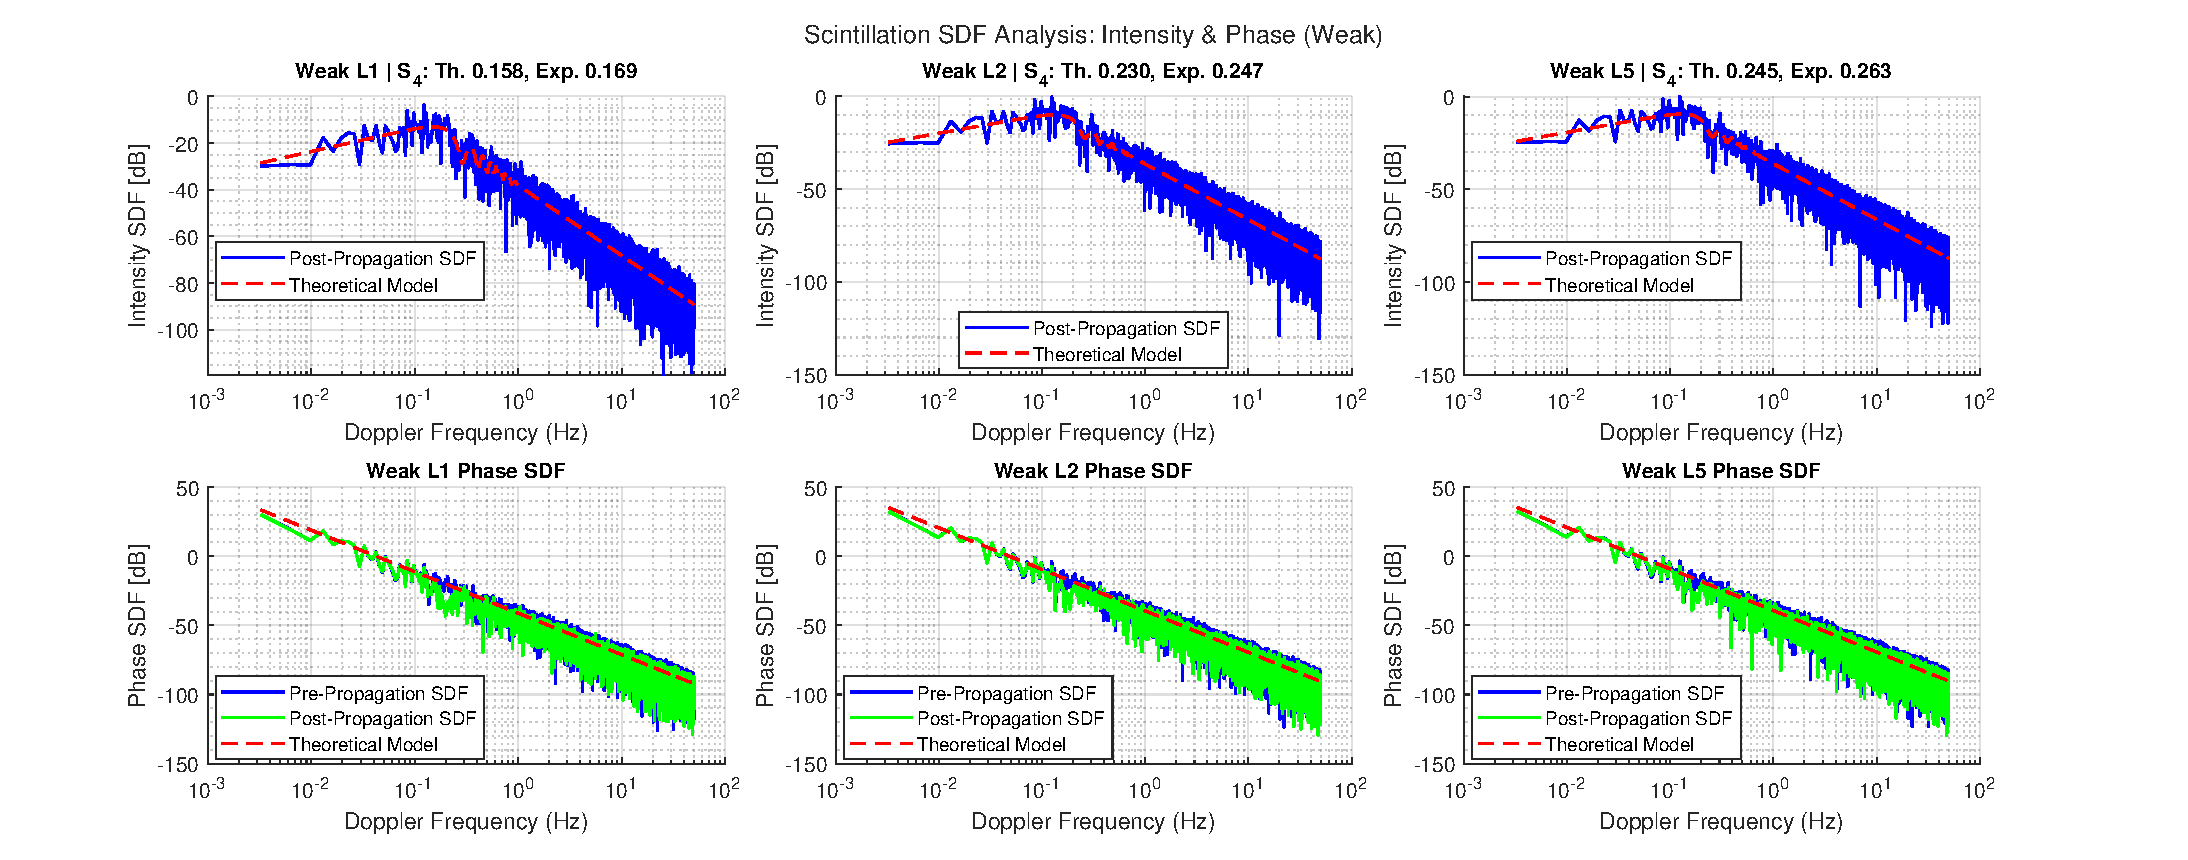
\includegraphics[width=\textwidth]{Weak_Scintillation_SDFs.pdf}
    \end{subfigure}
    \vspace{10pt} % Adjusts spacing between figures
    \begin{subfigure}[b]{\textwidth}
        \centering
        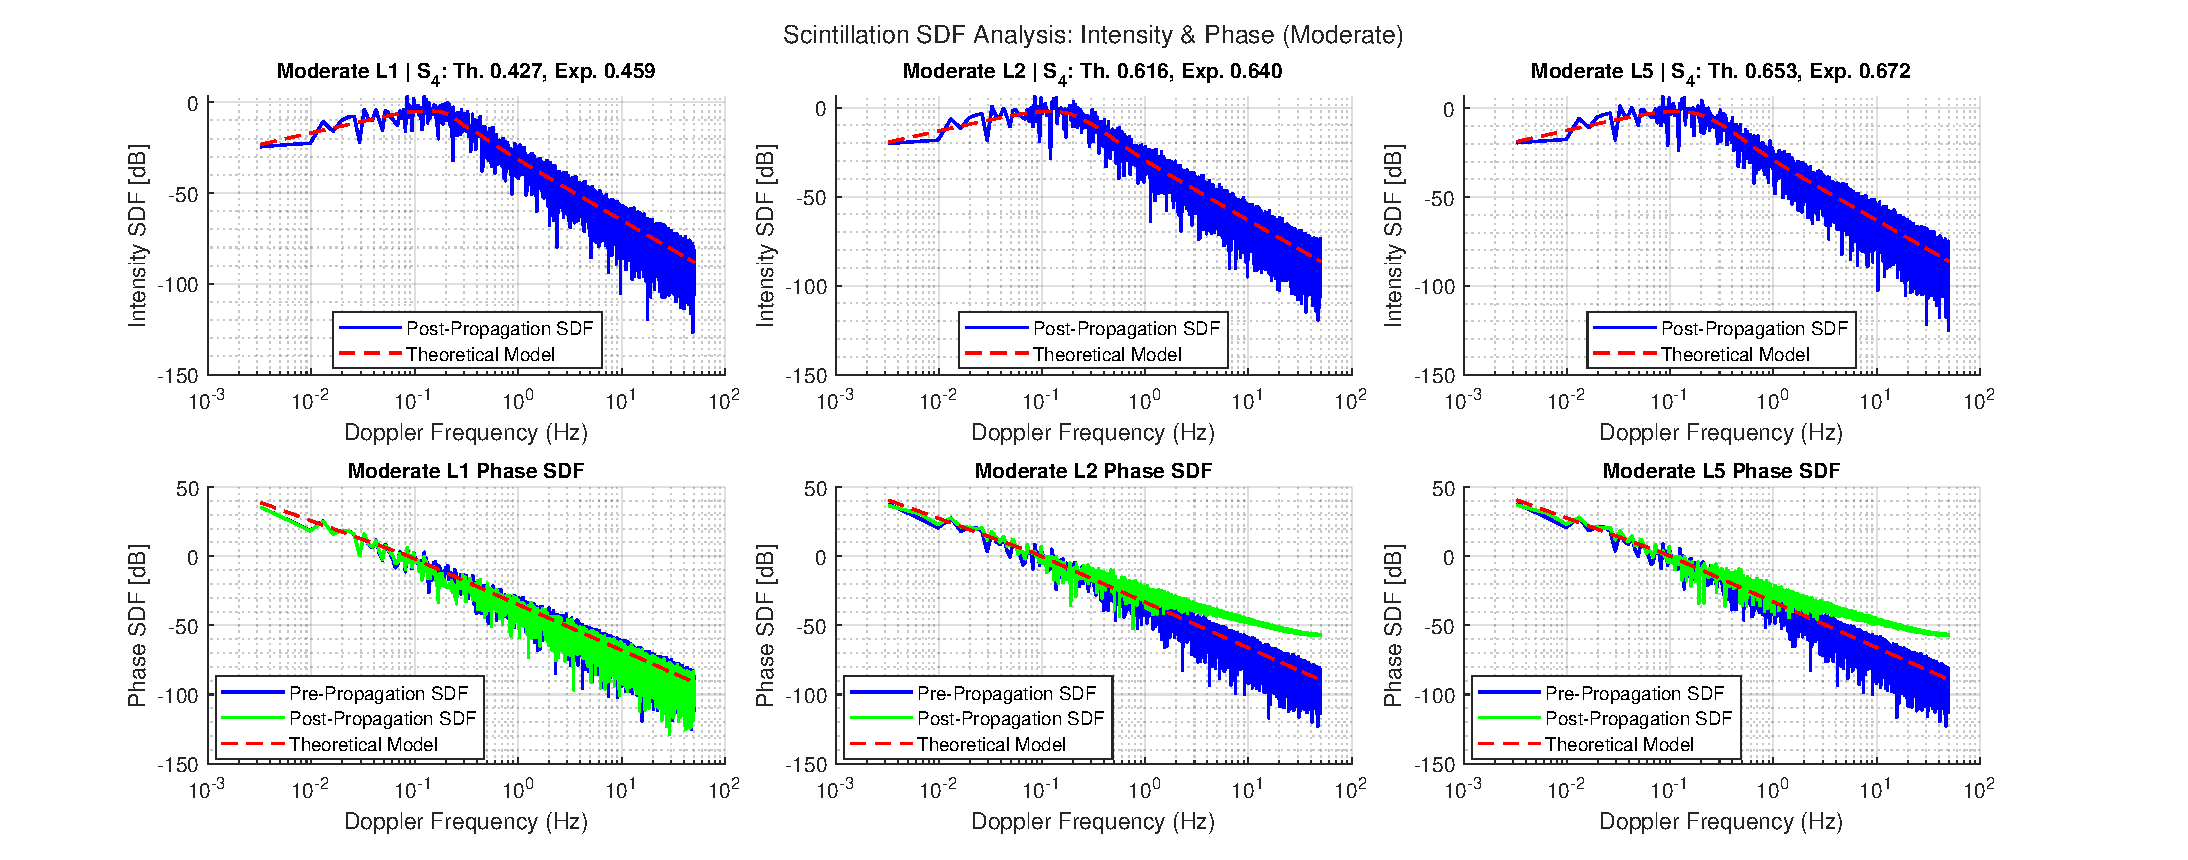
\includegraphics[width=\textwidth]{Moderate_Scintillation_SDFs.pdf}
    \end{subfigure}
    \vspace{10pt} % Adjusts spacing between figures
    \begin{subfigure}[b]{\textwidth}
        \centering
        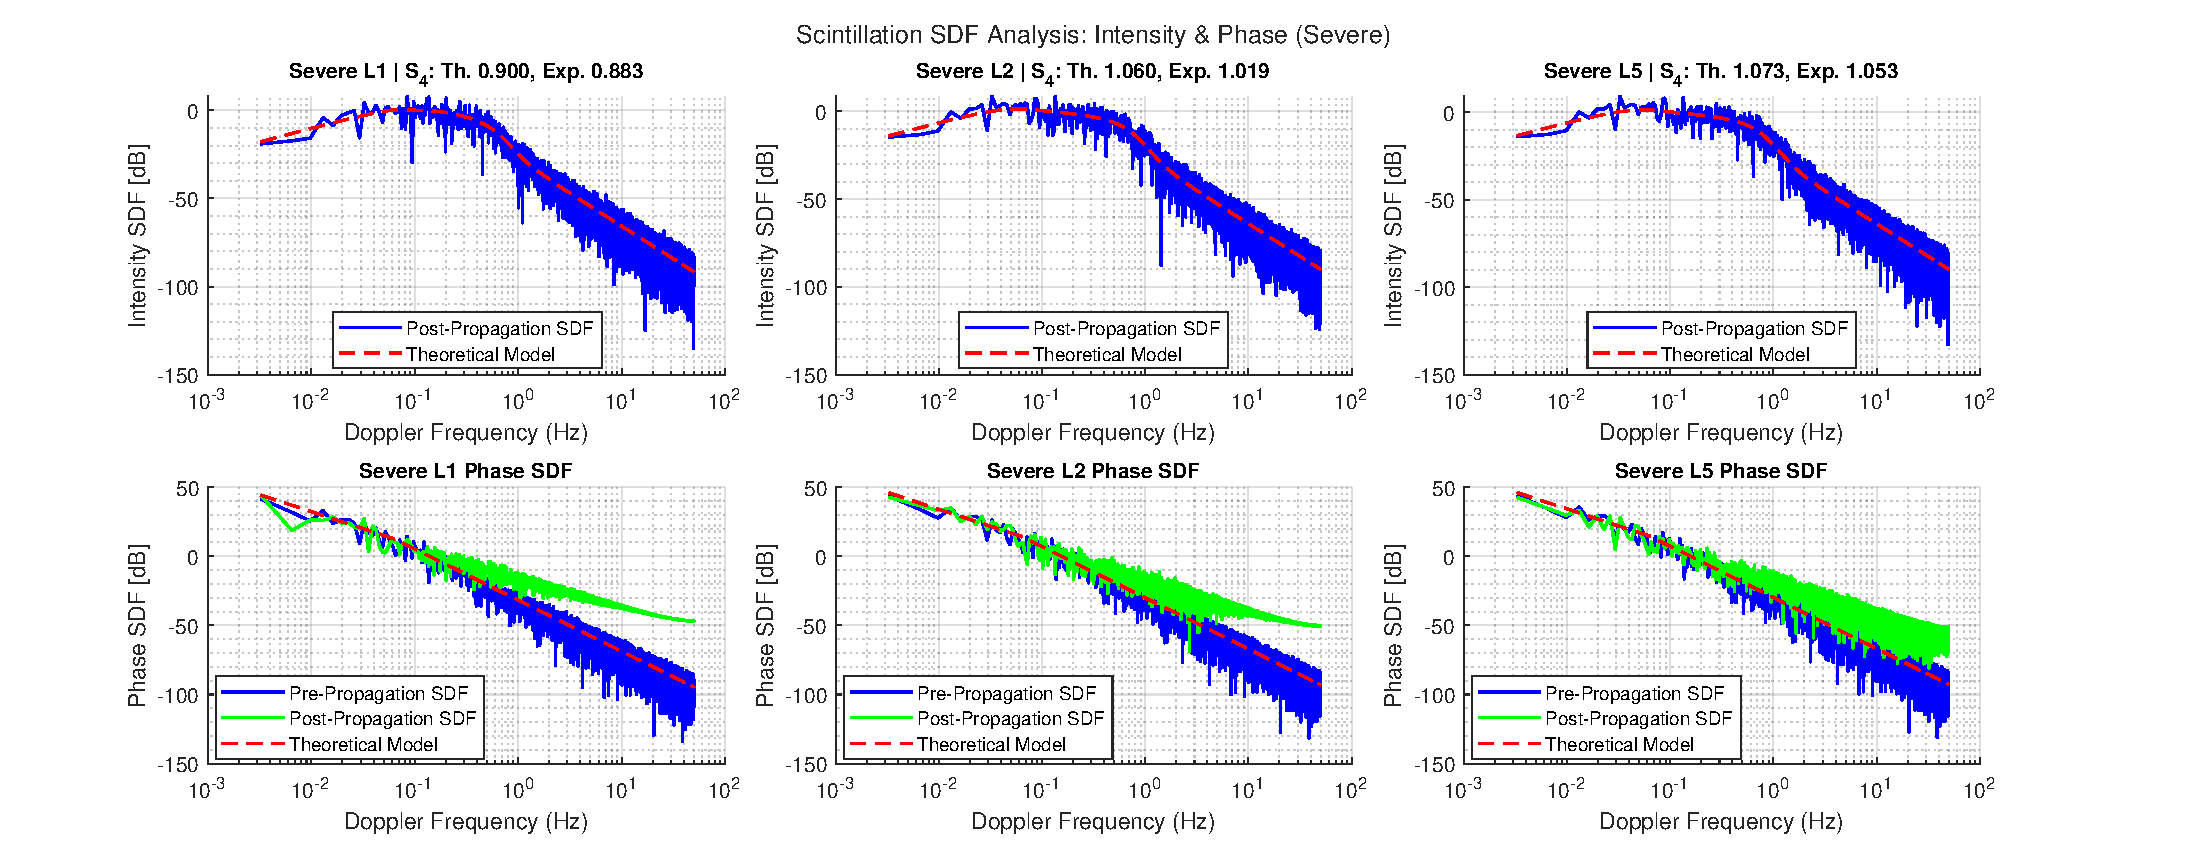
\includegraphics[width=\textwidth]{Severe_Scintillation_SDFs.pdf}
    \end{subfigure}
    \caption{This figure presents a comparison of spectral density functions (SDFs) for intensity and phase scintillation across three different severity levels: Severe, Moderate, and Weak. The analysis is performed for GPS L1, L2, and L5 frequency bands, arranged in a $2 \times 3$ grid for each severity case. The top row displays the Intensity SDF, where the blue line represents the post-propagation scintillation spectrum and the red dashed line corresponds to the theoretical intensity spectrum. The bottom row illustrates the Phase SDF, with the blue line showing the pre-propagation phase SDF, the green line indicating the post-propagation phase SDF, and the red dashed line representing the theoretical phase spectrum. The Severe case exhibits stronger spectral power and increased distortions, with significant deviations at high frequencies in the phase spectrum. The Moderate case presents an intermediate spectral behavior, while the Weak case follows the expected power-law trend with minimal deviations. These results highlight the impact of different scintillation severity levels on the signal’s intensity and phase, particularly emphasizing phase distortions in the post-propagation spectrum, which can lead to cycle slips and rapid phase oscillations, potentially affecting GNSS tracking loops. It is important to underpin that the experimental value of $S_4$ presents a statistical variability, which explains the slight discrepance of theoretical value. For further details on how these plots were obtained, please refer to \cite{githubGitHubRodrigodelimafgnssscintillationsimulator}}
    \label{fig:sdfs}
\end{figure*}

Furthermore, Figure \ref{fig:timeseries} present examples of the magnitude and phase time series of the propagated scintillation field for each scintillation severity level and frequency band considered for GPS applications. Although the current implementation only supports the L1, L2, and L5 GPS frequency bands, it can be easily modified to accommodate any GNSS frequency band.

Another noteworthy limitation of the simulator is that it currently only supports receivers moving in a rectilinear trajectory. To extend its capabilities, modifications would be required to allow the generation of scintillation time series for receivers with arbitrary trajectories. This enhancement would be particularly valuable for simulating scintillation effects on rockets, aircraft, and drone trajectories, among others.

\begin{figure*}[ht]
    \centering
    \begin{subfigure}[b]{\textwidth}
        \centering
        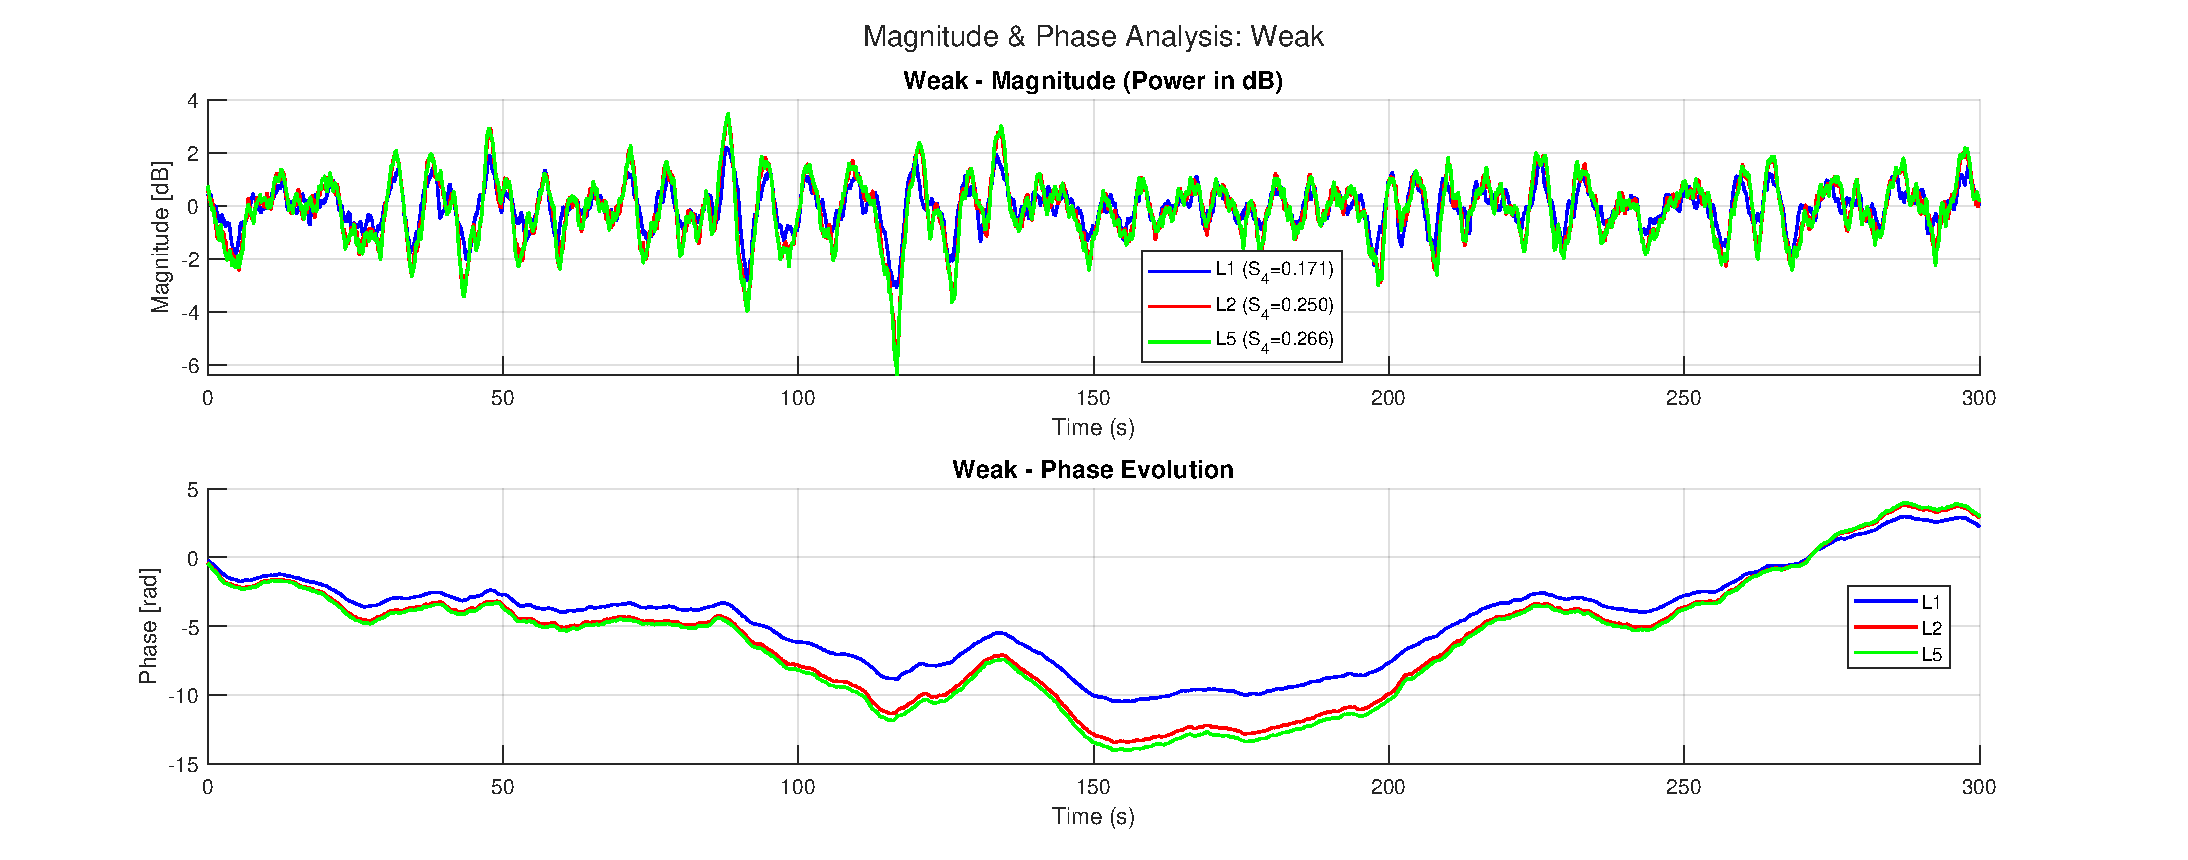
\includegraphics[width=\textwidth]{Weak_Magnitude_Phase_Time_Series.pdf}
    \end{subfigure}
    \vspace{10pt} % Adjusts spacing between figures
    \begin{subfigure}[b]{\textwidth}
        \centering
        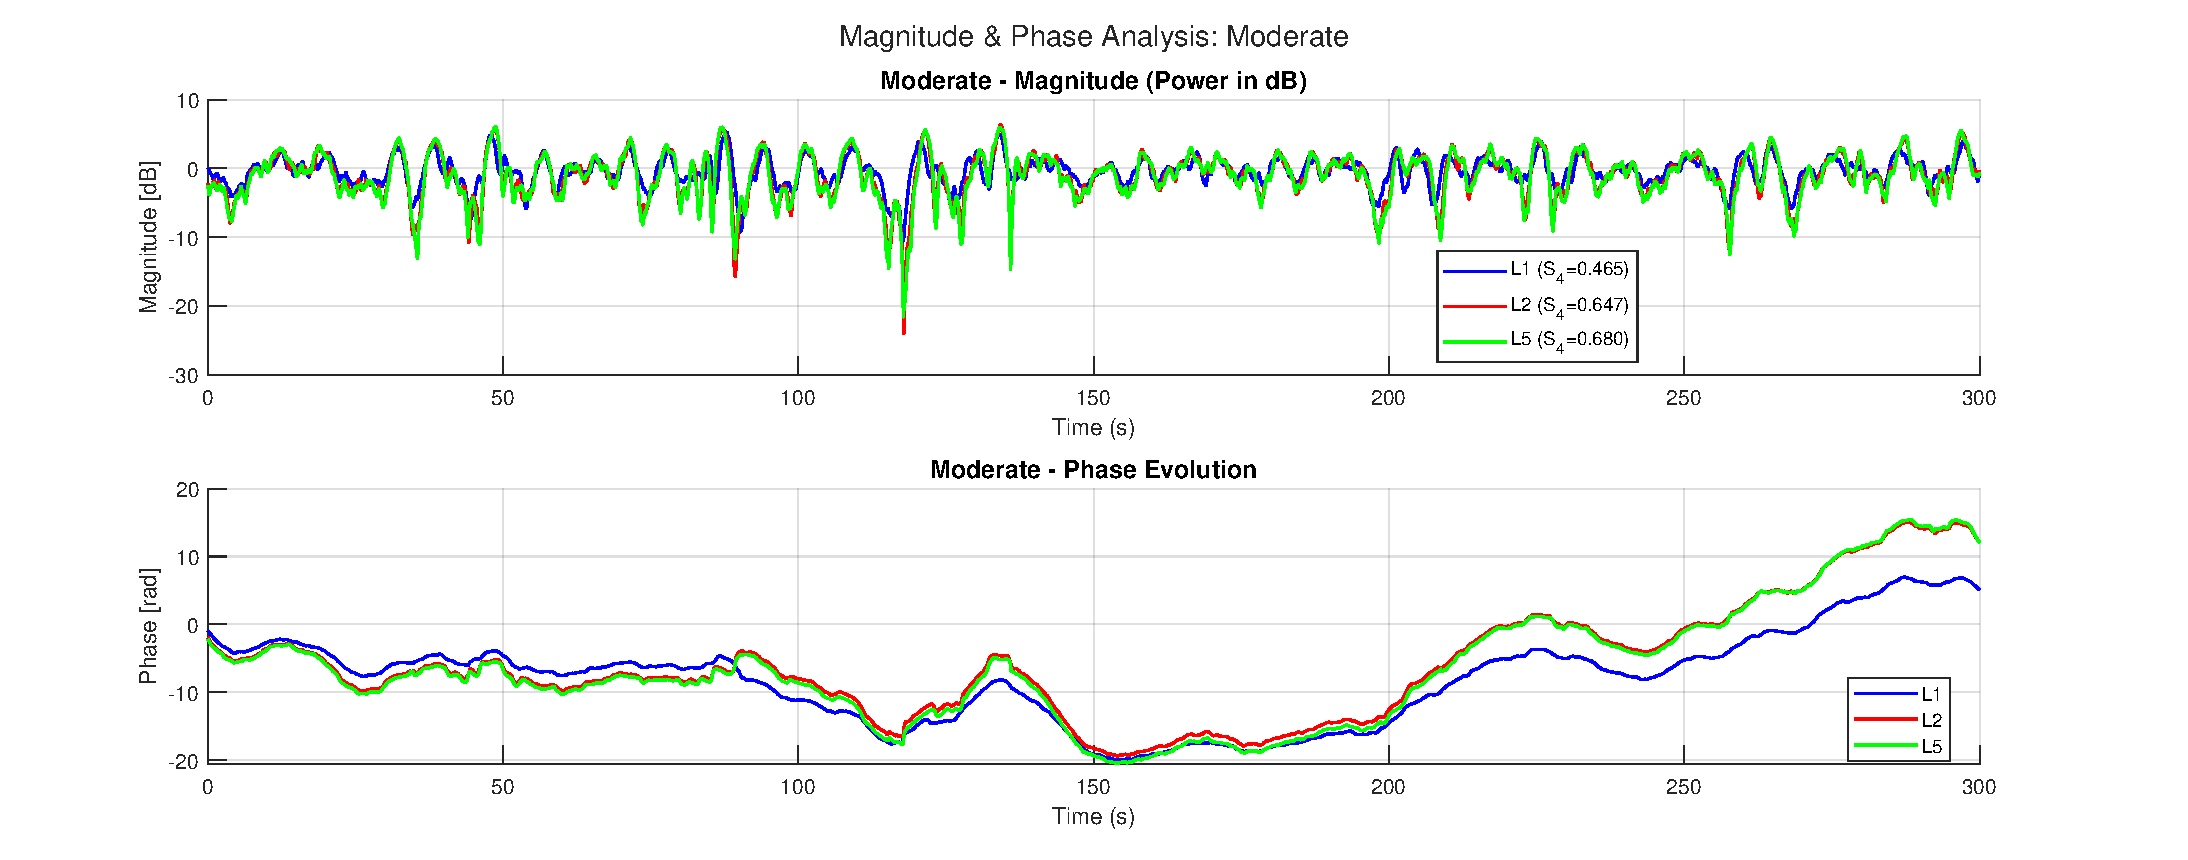
\includegraphics[width=\textwidth]{Moderate_Magnitude_Phase_Time_Series.pdf}
    \end{subfigure}
    \vspace{10pt} % Adjusts spacing between figures
    \begin{subfigure}[b]{\textwidth}
        \centering
        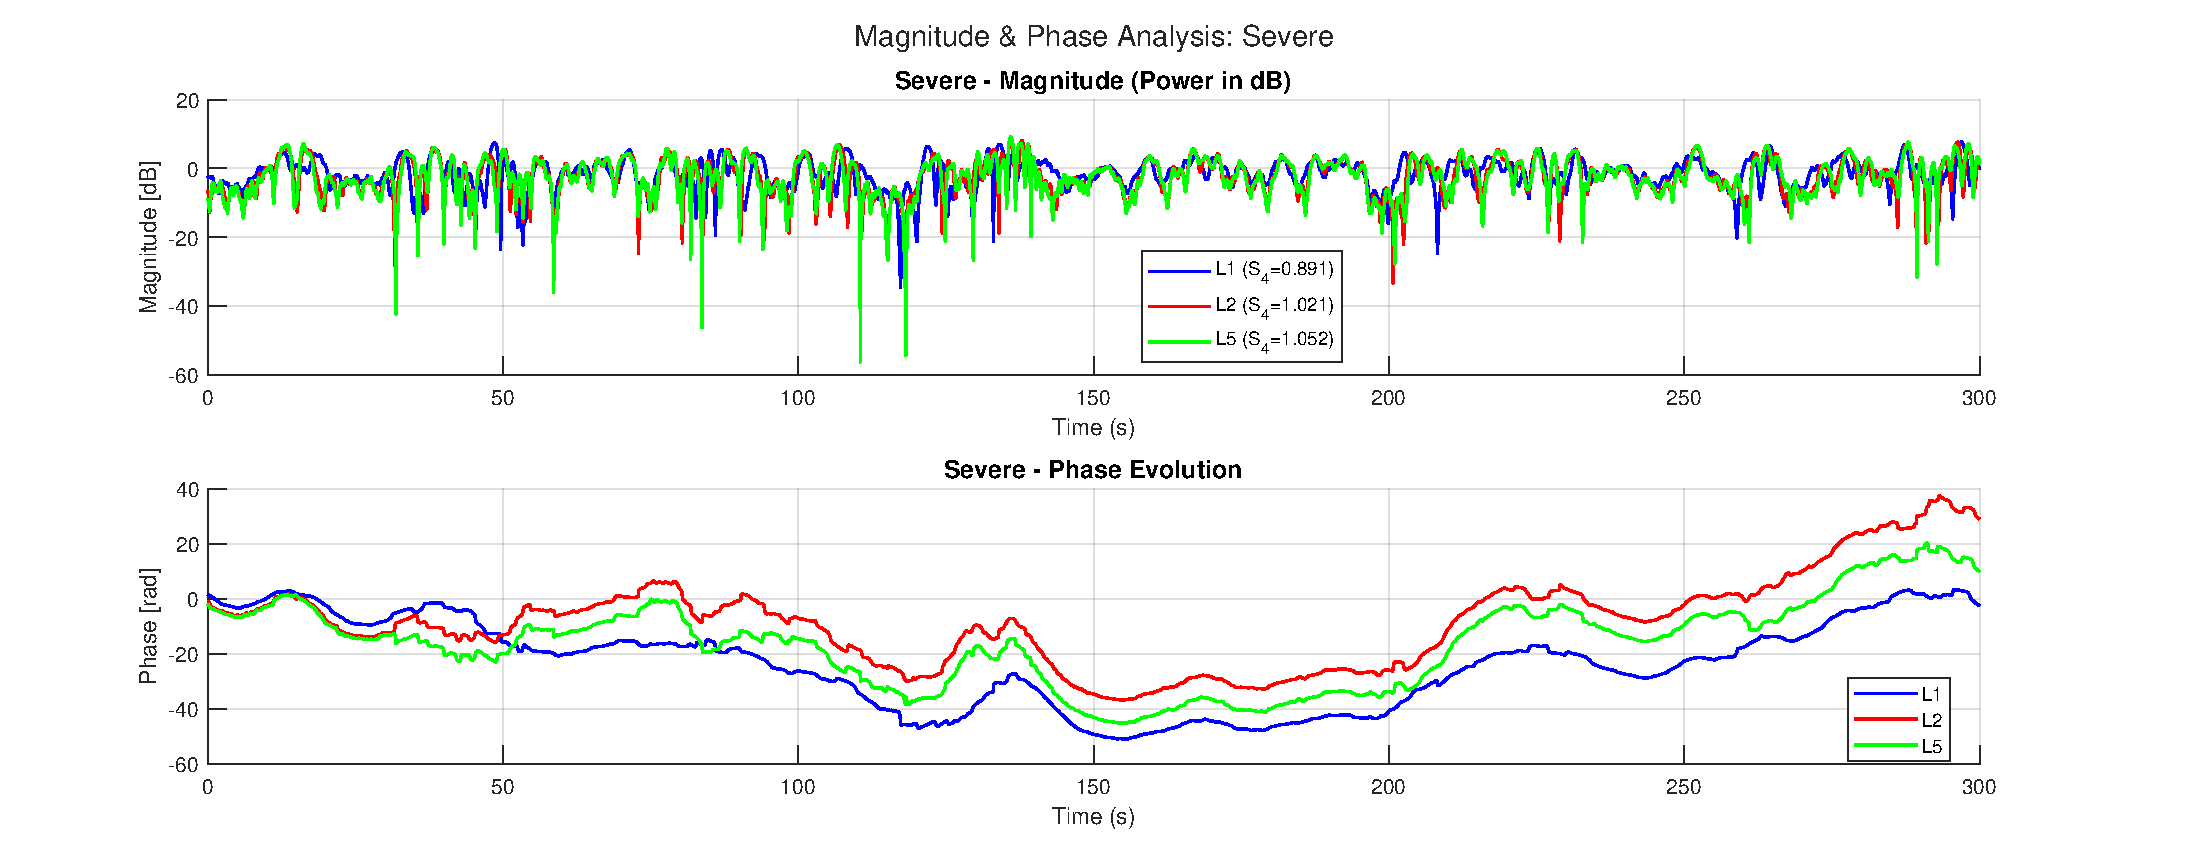
\includegraphics[width=\textwidth]{Severe_Magnitude_Phase_Time_Series.pdf}
    \end{subfigure}
    \caption{This figure presents the time series of signal magnitude (top row) and phase evolution (bottom row) for GPS L1, L2, and L5 frequency bands under different scintillation conditions: Severe, Moderate, and Weak. The magnitude is shown in dB as $10\log_{10}{\lvert \psi\left[ \rho_F; m \right]^{2} \rvert}$, while the phase in radians is computed as an unwrapped version of 2 quadrant arctangent of the imaginary and real parts of $\psi\left[ \rho_F; m \right]$. The colors represent different frequencies: blue (L1), red (L2), and green (L5). The top row illustrates the power fluctuations of the scintillation-affected signal, where higher scintillation severity leads to stronger amplitude fading. The bottom row shows the phase evolution, where increased scintillation severity causes larger phase variations, which may lead to cycle slips and phase tracking difficulties in GNSS receivers. The computed $S_4$ indices, displayed in the legend, quantify the scintillation strength for each frequency band. For further details on how these plots were obtained, please refer to \cite{githubGitHubRodrigodelimafgnssscintillationsimulator}}
    \label{fig:timeseries}
\end{figure*}

\section{A Generic Methodology for Generating Ionospheric Scintillation Time Series Using the TPPSM}
\label{sec:time_series_methodology}
In order to generate meaningful synthetic ionospheric scintillation time series using the refactored version of the TPPSM, one can following methodology:

\begin{enumerate}
    \item Set the initial position and velocity of a receiver.
    \item Set the date and time of the simulation in UTC.
    \item Choose a available satellite in line-of-sight.
    \item Set the mean drift velocity of the ionosphere in the eastward direction, which generally spans within the range of $\left[ 25, 125 \right]$ meters per second. This parameter directly affects the value of $\rho_F / v_{eff}$, which is tightly related to the intensity decorrelation time $\tau_0$.
    \item Set the lenght of the simulation time. In general, the most common time window used in the literature to analyze real data is around 300s \cite[Figure 2]{xuTwoparameterMultifrequencyGPS2020}, \cite[Figure 3]{JiaoScintillationOnGPSSignalsForDynamicPlatforms2018}.
    \item Set the sampling rate of the simulation. High frequency real data in general are obtained at 100 Hz \cite[Section 5]{xuTwoparameterMultifrequencyGPS2020}, \cite[Section IV, subsection A]{JiaoMultifrequencyScintillationOnGPSSignalsStaticPlatforms2018}.
    \item Choose a set of the irregularity parameters $\left\{ U, \mu_0, p_1, p_2 \right\}$ that resembles a Weak, Moderate or Severe scattering regime.
    \item Extrapolate the chosen irregularity parameters for multiple frequency bands if needed.
    \item Set a simulation seed.
    \item Simulate.
\end{enumerate}

For generating ionospheric scintillation time series for dynamic applications, where the receiver could move in any direction, we may follow the idea proposed in \cite[Figure 4]{JiaoScintillationOnGPSSignalsForDynamicPlatforms2018}, where the receiver velocity was configured in parallel and perpendicular directions with the alignment of the magnetic field.

It is important to emphasize here that the TPPSM present a extremely valuable tool in the hand of GNSS researchers who are trying to develop novel receiver technologies, given that it is a physics based model that relies on a well stablished statistical and geometrical characterization.

Therefore, the impact of the ionospheric scintillation, for any kind of scattering regime, on the following examples of applications can be directly assessed:

\begin{itemize}
    \item Ionospheric Scintillation Monitoring Stations
    \item Plane Landing Systems
    \item Drone Navigation
    \item Ballistic Rocket Missiles Navigation
    \item Agricultural Navigation
\end{itemize}
\section{Conclusions}
\label{sec:conclusions}

This study has successfully synthesized key aspects of the Two-Component Power Law Phase Screen Model (TPPSM), consolidating information previously scattered across various journal articles, conference papers, and books. A new refactored implementation of the TPPSM was developed to address the limitations of existing publicly available codes, particularly the lack of support for simultaneous weak scattering regime simulations and the use of real satellite orbits. The new implementation features enhanced documentation, improved code organization, and increased flexibility for simulating different scintillation severity levels.

The validity of the refactored TPPSM was rigorously assessed by comparing the intensity and phase spectra of simulated scintillation time series with their theoretical counterparts, confirming strong agreement across various scintillation conditions (Weak, Moderate, and Severe). The results demonstrated that the refactored model accurately reproduces expected spectral characteristics, including the phase distortions caused by free-space propagation, which are known to impact GNSS receiver tracking performance.

Furthermore, this study has proposed a systematic methodology for generating synthetic ionospheric scintillation time series using the TPPSM. The methodology allows researchers to configure simulation parameters based on satellite-receiver geometry, ionospheric drift velocity, and appropriate irregularity parameters for different scattering regimes. Additionally, an extrapolation approach was outlined to scale the model parameters across multiple frequency bands, ensuring compatibility with multi-frequency GNSS signals.

Despite these advancements, some limitations remain. The current implementation only supports rectilinear receiver motion, which restricts its applicability to dynamic platforms with arbitrary trajectories, such as aircraft, rockets, and drones. Future work should aim to extend the model to accommodate more complex receiver dynamics, enabling a broader range of GNSS applications.

The TPPSM remains a valuable tool for ionospheric scintillation research, particularly for evaluating the performance of GNSS receivers under different scintillation conditions. The insights from this study are expected to support the development of robust mitigation strategies, improve ionospheric monitoring techniques, and contribute to navigation system resilience in challenging environments.

Future efforts should focus on:
\begin{itemize} \item Enhancing the model to incorporate arbitrary receiver trajectories for dynamic platforms.
\item Investigating alternative irregularity parameter estimation techniques, including data-driven and machine learning approaches.
\item Expanding the model to include additional GNSS frequency bands beyond L1, L2, and L5.
\end{itemize}

By addressing these challenges, the TPPSM can continue to serve as a fundamental simulation tool for researchers working on ionospheric scintillation characterization, GNSS signal processing, and space weather effects on satellite-based navigation systems.

%----------------------------------------------------------

\printbibliography

%----------------------------------------------------------

\end{document}